% Dr. Nam H. Le. drnamlabs.com, bunnyquant.com
%% Neurocomputing (Elsevier) submission. Compile: pdflatex x2
\documentclass[preprint,12pt,authoryear]{elsarticle}

\usepackage{amsmath,amssymb,amsthm}
\newtheorem{proposition}{Proposition}
\usepackage{graphicx}
\usepackage[hidelinks]{hyperref}
\usepackage[T1]{fontenc}
\usepackage{lmodern}
\usepackage{microtype}
\usepackage{lineno}
\graphicspath{{figures/}}
\newcommand{\figwidth}{\linewidth}

\journal{Neurocomputing}

\begin{document}

\begin{frontmatter}

\title{Attention that eats itself: self-reference flattens the energy
landscape of modern Hopfield networks and transformer attention}

\author{Nam H. Le}
\ead{nam.le@uvm.edu}
\affiliation{organization={Department of Computer Science and Vermont Complex Systems Institute, University of Vermont},
            city={Burlington},
            state={VT},
            postcode={05405},
            country={USA}}

\begin{abstract}
Modern Hopfield networks give attention an energy: one retrieval step of a
dense associative memory with log-sum-exp energy is exactly the transformer
attention operation. Work built on this identity treats the energy landscape
as fixed at inference time, yet machine-learning systems increasingly read
from stores populated by their own outputs. I show that when a modern
Hopfield network, and therefore an attention head, overwrites its stored
patterns with its own retrievals, its energy landscape flattens one way.
Because every retrieval is a convex combination of stored patterns, some
contraction is guaranteed; what I measure is where it ends, how fast it
proceeds and how the landscape dies: basins merge in a cascade until a
single minimum remains near the data mean, attended uniformly. Pattern separation, the source of exponential capacity,
sets only the pace of this flattening, never its endpoint. On twelve
pretrained BERT heads, self-reference drives every head to the
uniform-attention fixed point, and a head's initial regime predicts how long
it resists; the basins disappear before the stored patterns finish
travelling. The endpoint coincides with depth-wise rank collapse, reached
here along time rather than depth. Energy-based selection over basin widths
delays the collapse, and averts it only when the stored patterns encode a
problem whose structure retrieval can exploit, in which case the same loop
discovers optima it was never shown. Capacity is a clock, not a shield.
\end{abstract}

\begin{keyword}
modern Hopfield networks \sep dense associative memory \sep transformer
attention \sep energy landscape \sep model collapse \sep rank collapse
\end{keyword}

\end{frontmatter}

\linenumbers

\section{Introduction}

Dense associative memories extended the classical Hopfield network
\citep{hopfield1982} with sharper interaction functions, buying a
storage capacity that grows polynomially \citep{krotov2016} and then
exponentially \citep{demircigil2017} in dimension. \citet{ramsauer2021}
closed the circle with an exact identity: for the log-sum-exp energy, one
step of the retrieval dynamics \emph{is} the attention operation of the
transformer \citep{vaswani2017},
\begin{equation}
\xi^{\mathrm{new}} \;=\; X\,\mathrm{softmax}\!\left(\beta X^{\top}\xi\right)
\;\;\equiv\;\;
z \;=\; V\,\mathrm{softmax}\!\left(\tfrac{1}{\sqrt{d}}K^{\top}q\right),
\label{eq:identity}
\end{equation}
with stored patterns $X$ as keys and values, query pattern $\xi$ as the
incoming token, and inverse temperature $\beta$ as $1/\sqrt{d}$
(Fig.~\ref{fig:identity}a). The identity has since become constructive:
entire transformer blocks have been derived from a single global energy
function \citep{hoover2023}, energy minimization has been proposed as the
substrate of inference-time reasoning \citep{gladstone2025}, and diffusion
models have been recognized as dense associative memories whose spurious
minima are the first signatures of generalization \citep{pham2025}.

All of this work shares one assumption: the landscape stands still. The
memories are written by training, and inference only descends the energy
they define. But a second literature has been documenting what happens when
learning systems consume their own outputs. Generative models retrained on
their own samples degrade \citep{shumailov2024, alemohammad2024}, with the
severity governed by whether synthetic data replaces or merely accumulates
alongside real data \citep{gerstgrasser2024, bertrand2024}; iterated
learning in humans converges to the prior of the learner rather than the
structure of the data \citep{griffiths2007}. And a small literature
descending from \citet{watson2011} has studied classical Hopfield networks
that relearn their \emph{own attractors}, finding that such
``self-modeling'' can enlarge the basins of good minima, a line recently
reviewed by \citet{froese2025}, entirely within the classical,
quadratic-energy setting. Closer to modern Hopfield networks, unlearning
schemes that let a network reshape its stored patterns using its own
attractors can improve retrieval \citep{serricchio2025}, and replay
selected by Hopfield energy has been proposed to limit forgetting when a
memory is retrained \citep{takeda2026}; in both, the stored set is shaped
by an external procedure rather than overwritten by the network's own
retrievals.

A third literature has already found the endpoint I will describe, by a
different road. Stacking attention layers drives token representations
toward a rank-one configuration in which attention is uniform: pure
attention loses rank doubly exponentially with depth
\citep{dong2021}, rank collapse impairs signal propagation and
trainability \citep{noci2022}, the tokens of a deep self-attention flow
cluster and eventually merge \citep{geshkovski2025}, and masks and
normalization only change how fast this happens \citep{wu2024}. In all of
these the weights and the context are fixed and the collapse unfolds
along \emph{depth}, within a single forward pass. Here nothing is stacked:
one head, with its pretrained weights, reads from a memory that it
gradually rewrites, so the collapse unfolds in \emph{time}, across
rounds of storage. That two different dynamics share the same
uniform-attention endpoint is itself part of what I report.

These two literatures have not met. What self-reference does to a
\emph{modern} Hopfield network, and therefore, through
identity~(\ref{eq:identity}), to an attention head, has to my knowledge
not been characterized, even though the attention head is precisely the
place where modern systems most literally read from stores their own
outputs may later populate. Retrieval-augmented systems write generated
answers back into the document stores they retrieve from; agents with
external memory store their own summaries and reread them; and corpora
used to train the next model increasingly contain text produced by the
last. In each case a memory that is read by attention is partly written
by the reader. This paper makes the characterization, in the
field's own vocabulary and partly on the field's own artifacts. My
retrieval operator is bit-identical (maximum deviation $2\times10^{-14}$) to
the reference implementation accompanying \citet{ramsauer2021}, and my main
experiment runs on pretrained \texttt{bert-base-uncased} heads, measured
with the same statistic \citet{ramsauer2021} used to classify real attention
heads along the regime axis from \emph{selective retrieval} to \emph{global
averaging}.

Part of the answer follows from geometry alone. A retrieval is a convex
combination of stored patterns, so a memory that only ever stores its own
retrievals can never leave the convex hull of what it started with, and
must contract (Proposition~\ref{prop:hull}). The questions geometry leaves
open are the ones this paper answers empirically: where inside the hull
the memory ends, how fast it gets there, what happens to the basins of
attraction on the way, and what it takes to escape.

I find a single organizing picture (Fig.~\ref{fig:identity}b,c). A
self-referential attention memory flows one-way along the regime axis to a
universal fixed point: a flat landscape with one surviving minimum near the
data mean, attended uniformly. Sharpness (Krotov's interaction exponent
$n$, the softmax temperature $\beta$, a multiplier $\tau$ on pretrained
logits) changes only the clock. A positive control shows the escape
route: when stored patterns encode a problem with structure to exploit and
retrieval is biased so that better memories sit in wider basins, the same
loop climbs instead of collapsing, ending beyond everything it was ever
shown.

\begin{figure}[t]
\centering
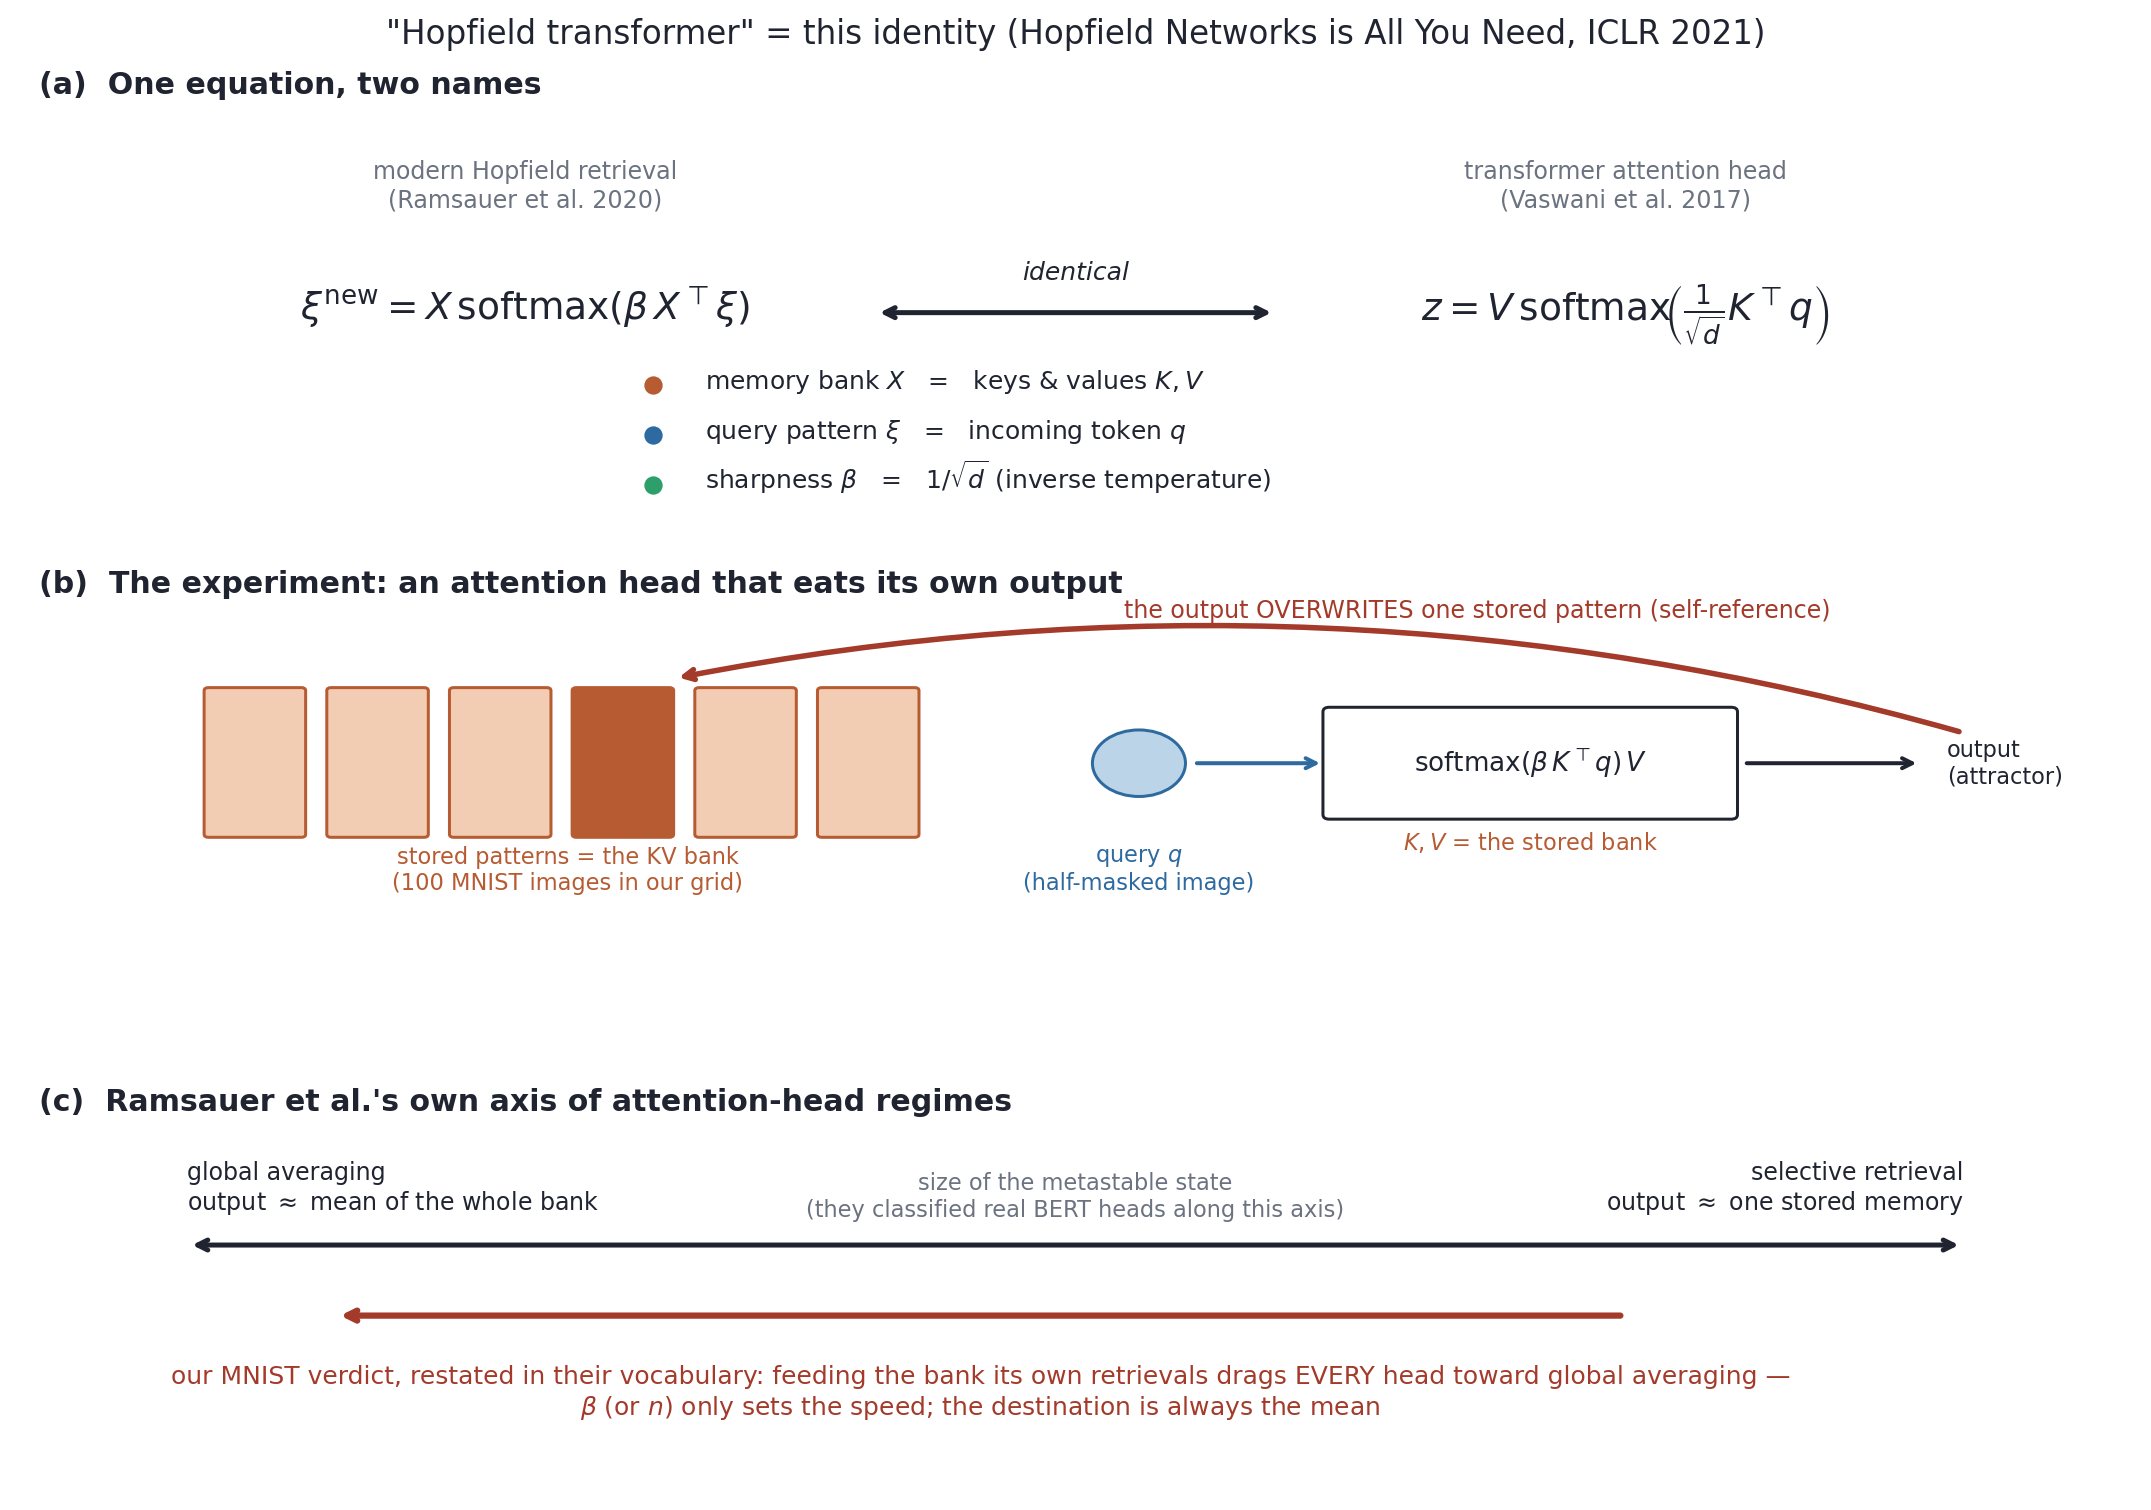
\includegraphics[width=\figwidth]{hopfield_is_attention}
\caption{\textbf{The object under study.} (a)~One retrieval step of a
modern Hopfield network is the attention operation
\citep{ramsauer2021}. (b)~The self-reference loop: the retrieval output
overwrites one stored pattern of the key--value bank; iterating couples the
energy landscape to its own minima. (c)~\citet{ramsauer2021} classify
attention heads along one axis, from global averaging to selective
retrieval, by the size of the metastable state. My result, stated on their
axis: self-reference drags every head toward the averaging endpoint, at a
speed set by sharpness and starting position.}
\label{fig:identity}
\end{figure}

\section{Results}

\subsection{One operation, three substrates}

All experiments iterate the same loop. A bank of $K$ stored patterns is
queried with a fresh probe; the retrieval output (a
softmax- or power-weighted mixture of the stored patterns,
Eq.~(\ref{eq:identity})) overwrites one randomly chosen slot of the
bank. Nothing else changes: no gradients, no learning rate, no objective.
The loop is run on three substrates of increasing realism: (i)~a
compositional spin-glass world where retrieval quality is externally
defined, (ii)~MNIST images under a pre-registered protocol, and (iii)~the
hidden-state banks of twelve pretrained BERT attention heads, retrieved
through their own learned projections. Throughout, every judgment of
quality or identity is made by an external referee (exact enumeration,
a 1-NN classifier on held-out real data, or frozen probe statistics), never
by the model's own energy.

The softmax arm of the loop is not an analogy to attention. I certify it
against the reference \texttt{Hopfield} layer released with
\citet{ramsauer2021}: with identity projections and matched scaling, the two
implementations agree to a maximum absolute deviation of $2\times10^{-14}$
across random banks and queries. Every result below is therefore a
statement about the attention operation itself.

\subsection{What the loop guarantees, and what it does not}

In the self-referential arms on MNIST and BERT, including the arms with a
basin bias, every write is $\xi^{\mathrm{new}}=\sum_i w_i x_i$ with
$w_i\ge0$ and $\sum_i w_i=1$ (for the power rule, a query with no positive
overlap receives uniform weights). This has a consequence that needs no
simulation.

\begin{proposition}\label{prop:hull}
Let $B_t=\{x_1,\dots,x_K\}$ be the bank at round $t$ and let each round
replace one slot by a convex combination of $B_t$. Then (i)~the convex
hull cannot grow, $\mathrm{conv}(B_{t+1})\subseteq\mathrm{conv}(B_t)$;
(ii)~no new extreme point is ever created, so an extreme point, once no slot
holds it, never returns; and (iii)~if all weights are strictly positive,
as for a softmax at finite $\beta$, the only banks left unchanged by every
possible write are those whose patterns all coincide.
\end{proposition}

\noindent\emph{Proof.} (i) and (ii): the written pattern lies in
$\mathrm{conv}(B_t)$, and removing a point from a set cannot enlarge its
hull. (iii): if the bank holds two distinct patterns it has an extreme
point $x_e$; a combination with strictly positive weights over at least
two distinct points is not an extreme point of the hull, so overwriting a
slot that holds $x_e$ changes the bank. $\square$

Self-reference without selection is therefore a consensus process in the
sense of \citet{degroot1974}: it can only lose diversity, and a single
repeated pattern is its only resting state. The proposition says nothing,
however, about four things, and these are what the experiments measure:
(a)~\emph{where} in the hull the bank ends (the mean of the data, a class
prototype, or an arbitrary stored pattern are all admissible);
(b)~\emph{how fast} it contracts, and what sets the clock; (c)~what happens
to the \emph{attractors} of the retrieval map, which are not the stored
patterns and can vanish long before the patterns meet; and (d)~what it
takes to \emph{escape}, which by the proposition requires a write that
leaves the hull. On the spin-glass substrate the write is followed by a
per-module binarization to the nearest valid composition, a non-convex
projection that can produce points outside the hull of the bank; this is
the only substrate on which the loop can, even in principle, discover.

\subsection{A positive control: when self-reference discovers}

\begin{figure}[t]
\centering
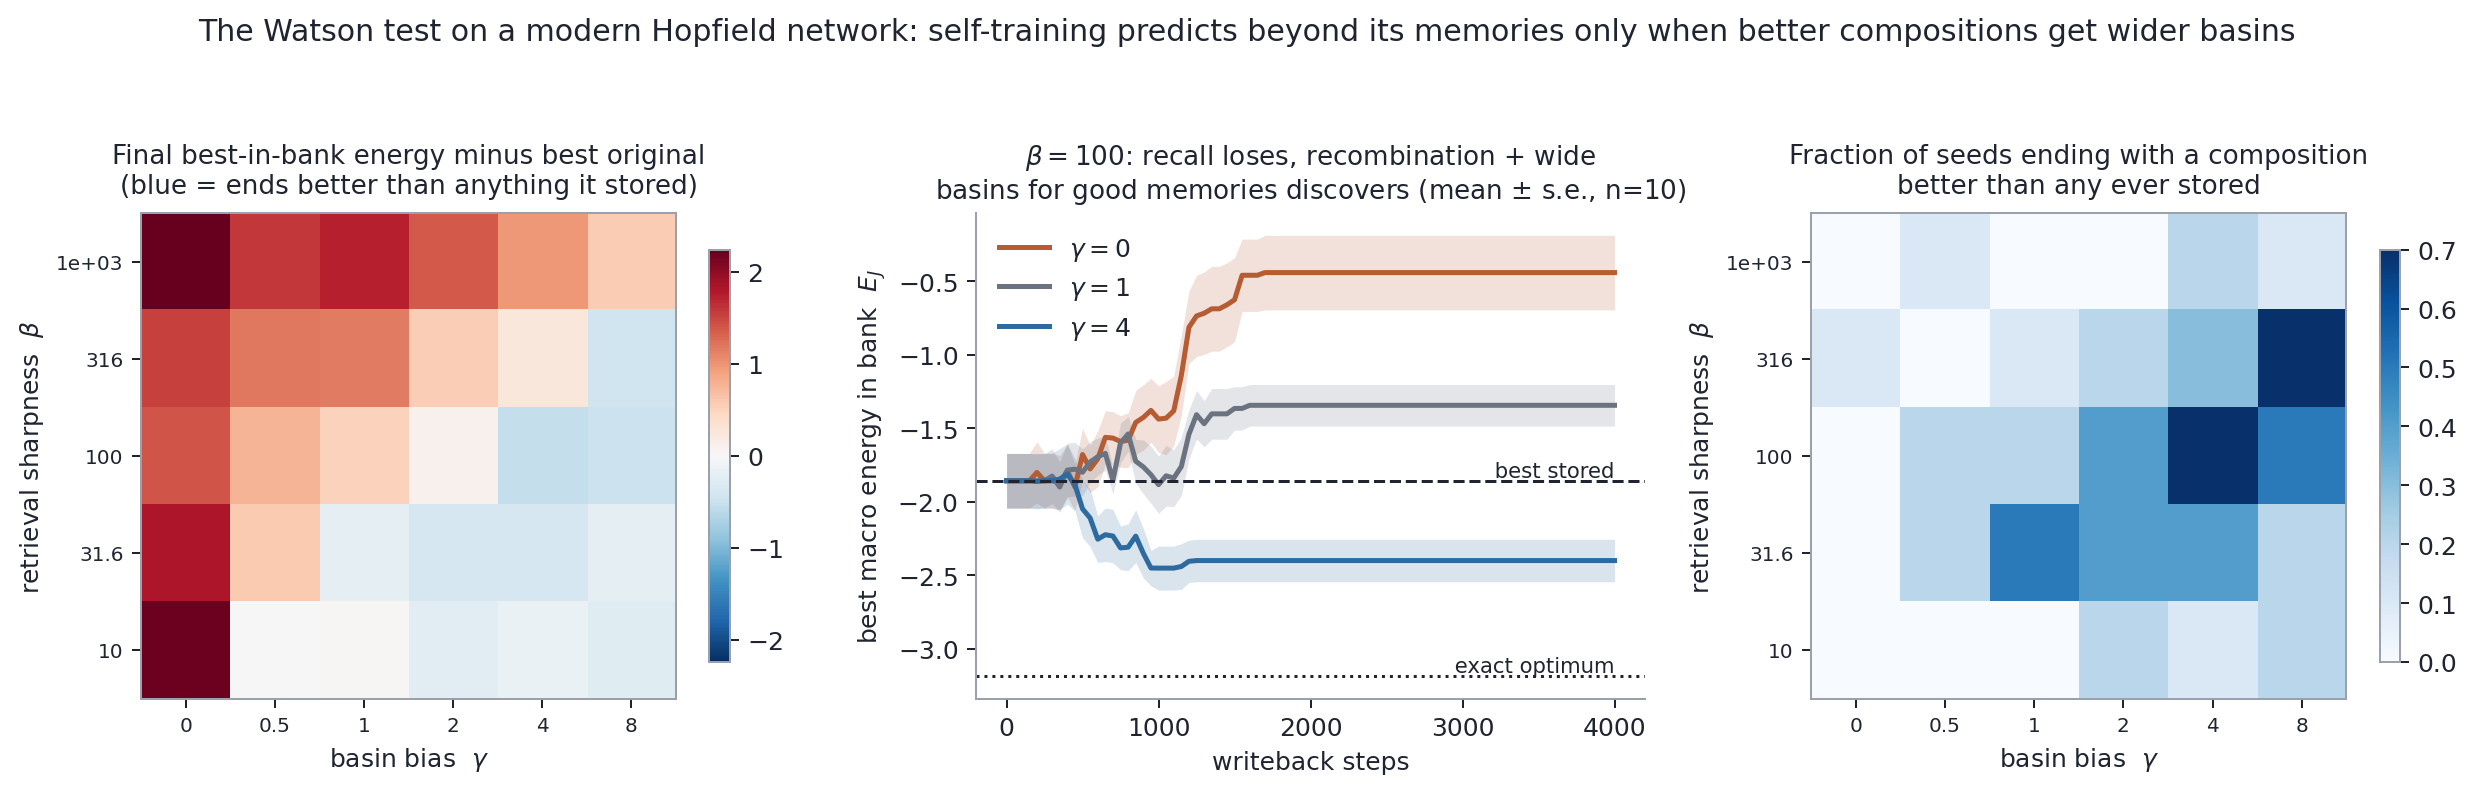
\includegraphics[width=0.78\figwidth]{watson_selection}
\caption{\textbf{Self-reference can discover, if quality buys basin
width.} Compositional spin-glass substrate. Pure self-training ($\gamma=0$)
is neutral drift: the bank explores novel compositions but fixates, ending
farther from the optimum than it began. Biasing retrieval logits by a
frozen problem energy ($-\gamma E_J$; better compositions get wider basins,
no accept/reject step) reverses the outcome: at moderate sharpness the bank
ends strictly better than anything it ever stored.}
\label{fig:watson}
\end{figure}

To know what collapse is, one must first see its alternative. On the
spin-glass substrate, patterns are compositions of module-level
configurations of a frustrated macro-problem, so each memory has an
externally defined energy $E_J$ and recombining memories can, in principle,
assemble optima never stored. Pure self-reference explores (the loop
writes dozens of novel valid compositions) but holds nothing: diversity
decays monotonically and the bank fixates, ending \emph{worse} than its
starting contents (median gap to the global optimum $1.33 \to \approx 3$).
This is neutral drift in the population-genetics sense: replacement without
selection.

The Watson ingredient \citep{watson2011}, translated from basin
\emph{relearning} into its modern form, is to let quality set basin
width: retrieval logits are biased by $-\gamma E_J$ with the problem
Hamiltonian frozen, so better compositions are easier to fall into, while
the dynamics remains pure retrieval. This flips the outcome
(Fig.~\ref{fig:watson}). At intermediate sharpness ($\beta\approx32$--$100$)
and $\gamma\approx2$--$4$, the bank ends better than anything it ever
stored in 40--70\% of seeds (gap $1.33\to0.79$; vs.\ $\gamma=0$:
Mann--Whitney $p=1.2\times10^{-4}$, Cohen's $d=3.0$; vs.\ the original
bank: Wilcoxon $p=.02$). At $\beta=1000$ retrieval degenerates into
copying, which can preserve but never predict: discovery lives in the
recombination regime, not the lookup regime.

\subsection{A pre-registered falsification on MNIST}

\begin{figure}[t]
\centering
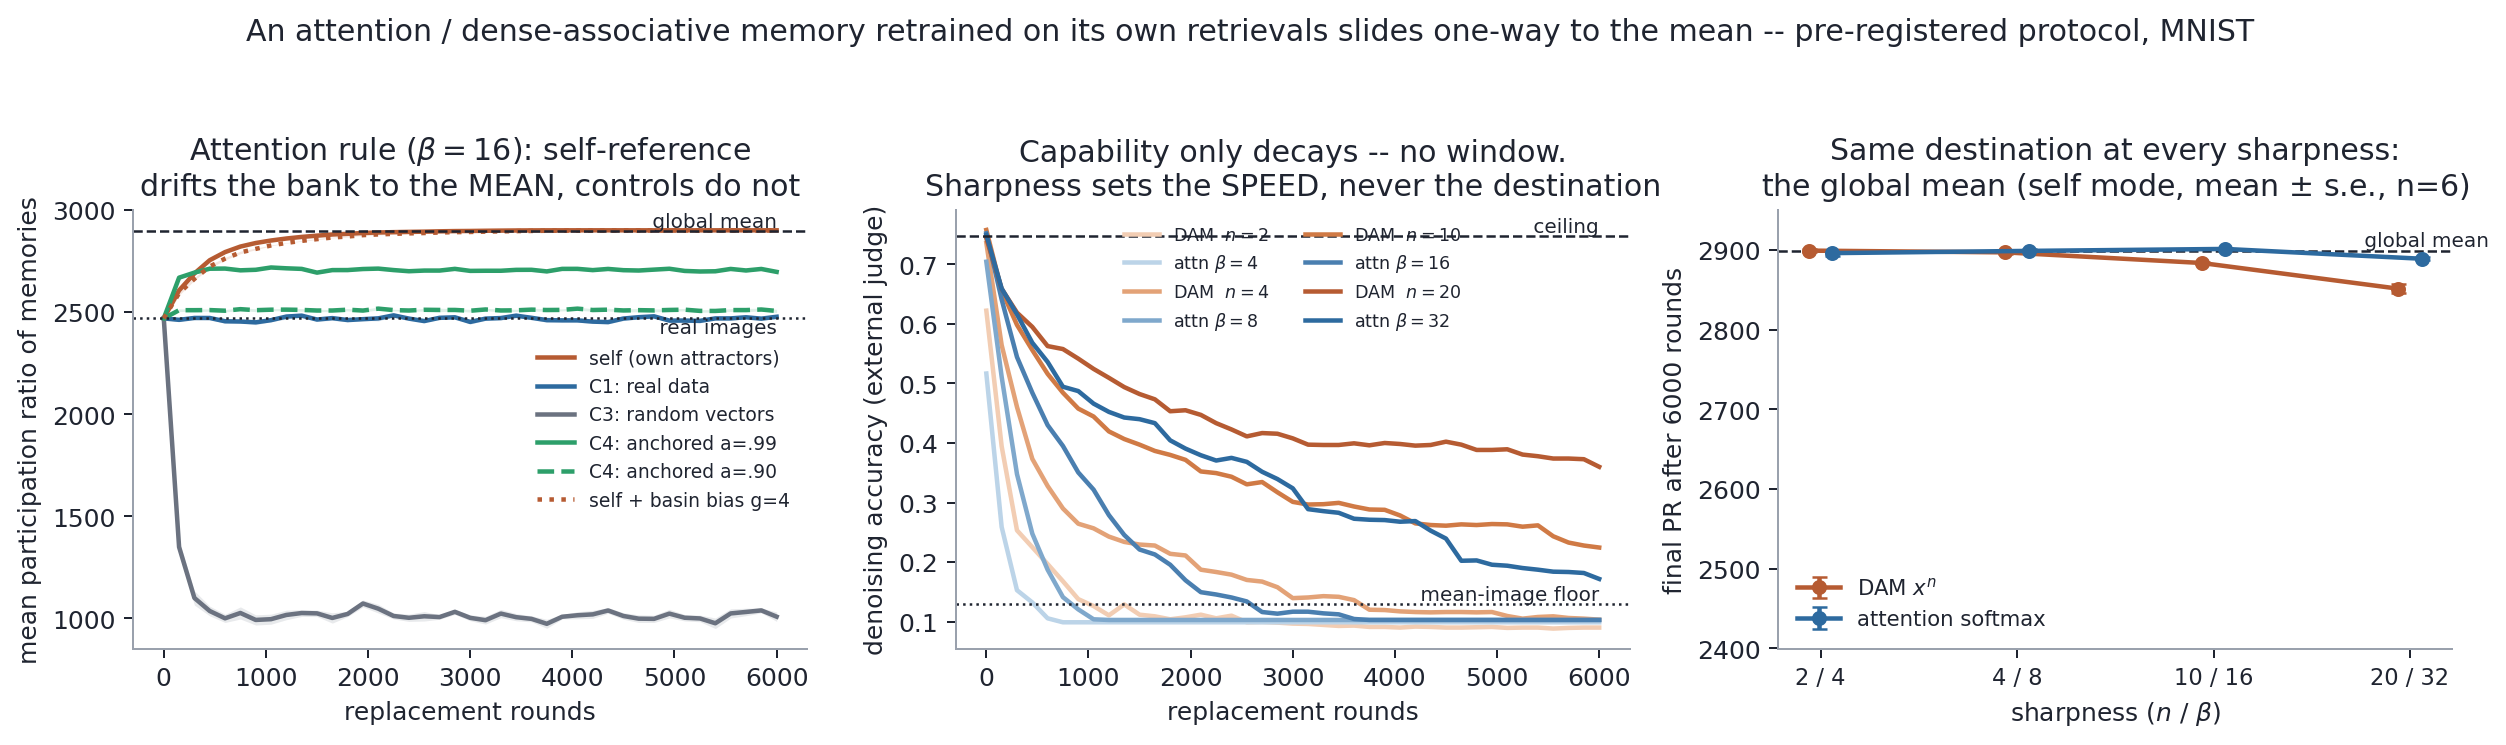
\includegraphics[width=\figwidth]{mnist_verdict}
\caption{\textbf{The drift is to the mean, not to prototypes.} (a)~Mean
participation ratio (PR) of the memories' correlation profiles under the
attention rule: self-reference drives the bank from the real-image level to
the global-mean level; replacing memories with fresh real images (C1) does
not move it. (b)~Denoising accuracy, judged by an external 1-NN classifier,
only decays; sharpness (DAM exponent $n$, attention $\beta$) sets the decay
rate. (c)~Final PR is independent of sharpness for both rules: same
destination, different clocks.}
\label{fig:mnist}
\end{figure}

Before the experiments were run, I wrote down a protocol with named
falsification criteria. The hypothesis~H, motivated by the
feature-to-prototype axis of dense associative memories \citep{krotov2016}
and by the memorization-to-generalization picture of \citet{pham2025},
predicted that a self-referential memory drifts toward \emph{prototypes}
(class-mean-like patterns), with the interaction exponent $n$ setting
the speed. A second hypothesis~H$'$ predicted a transient capability
window. Both died by their own pre-registered criteria, and the way they
died is the finding.

The bank (100 real MNIST images) does drift, and the drift is causally
self-referential: feeding fresh real images (control C1) holds the
participation-ratio statistic flat (2470$\to$2478), feeding random vectors
(C3) drives it in the \emph{opposite} direction, and anchoring toward the
original bank (C4) slows it monotonically with anchor strength. But the
destination is not the class prototypes (PR $\approx2717$): it is the
global mean of the data (PR $\approx2899$), reached at every $n$ and every
$\beta$ (Fig.~\ref{fig:mnist}a,c). Capability never peaks; it only decays
from the starting ceiling, faster for blunt rules (final denoising
accuracy $0.09$ at $n=2$ vs.\ $0.36$ at $n=20$ after 6{,}000 rounds;
Fig.~\ref{fig:mnist}b). The DAM power rule and the attention softmax rule
are empirically interchangeable throughout, a dynamical confirmation of
identity~(\ref{eq:identity}). And the basin bias that rescued the spin
glass does \emph{not} rescue MNIST: a mean-blurred image still scores high
data-likeness, so selection by similarity has nothing to push against.
Where the spin glass had structure to exploit, an at-ceiling representation
task has only entropy to lose.

\subsection{Real pretrained attention heads migrate to the
uniform-attention fixed point}

\begin{figure}[t]
\centering
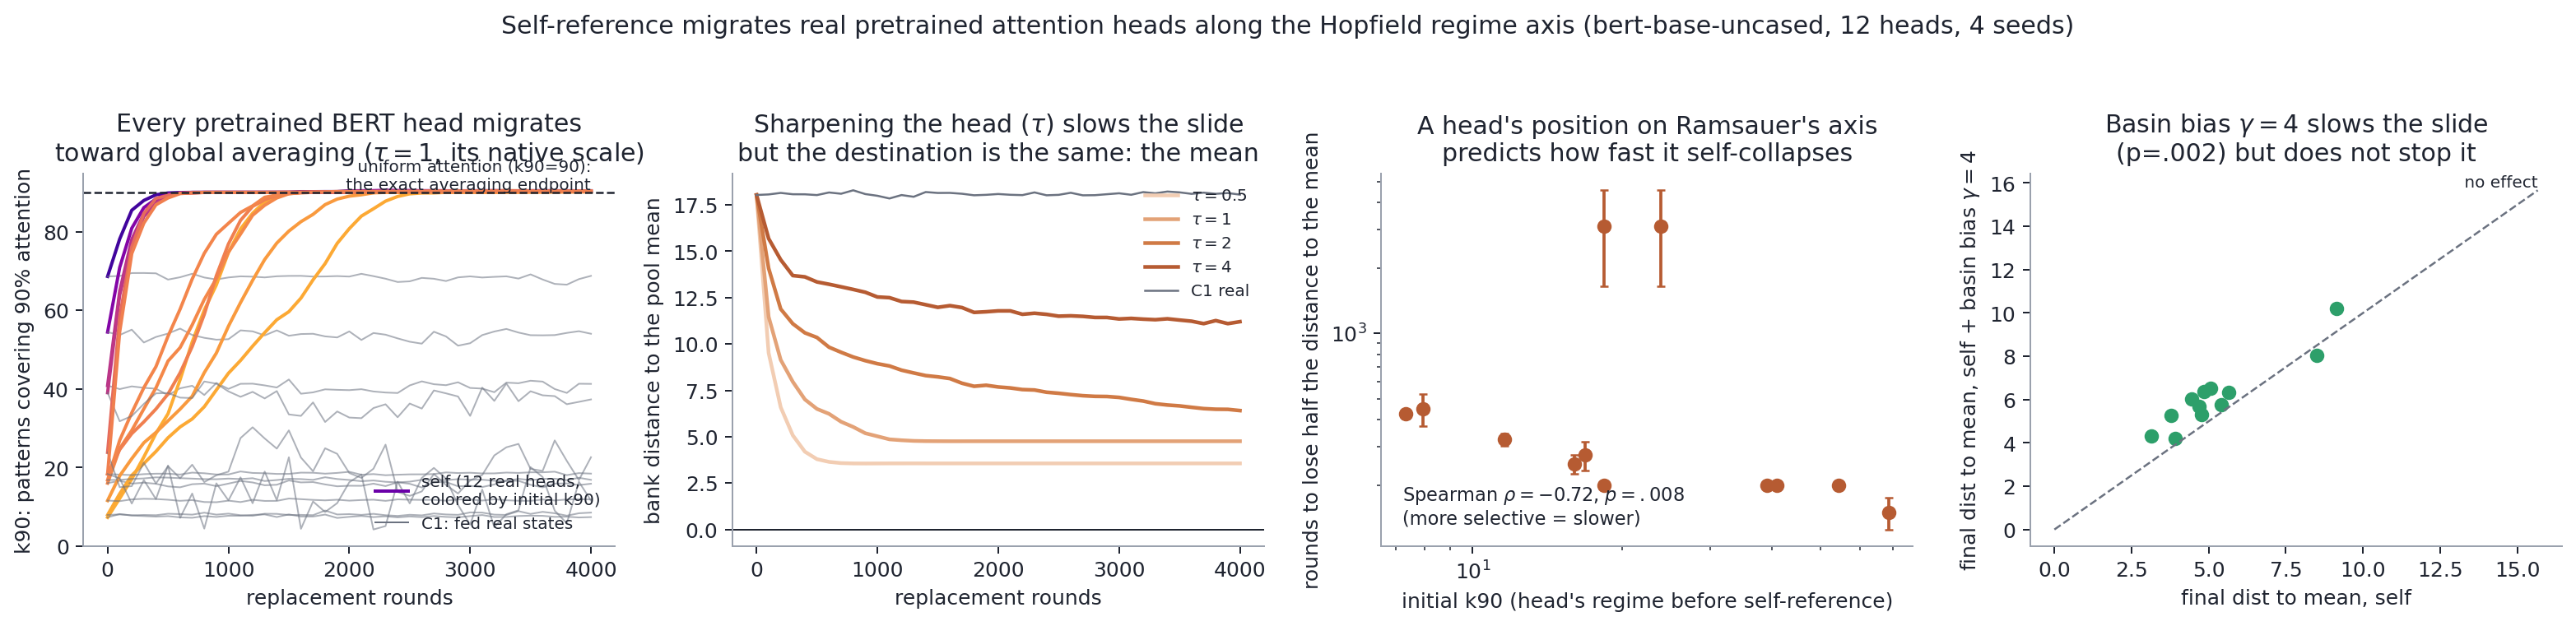
\includegraphics[width=\figwidth]{llm_regime_verdict}
\caption{\textbf{Twelve pretrained BERT heads under self-reference.}
(a)~$k_{90}$ (number of stored patterns covering 90\% of attention mass,
the metastable-size statistic of \citet{ramsauer2021}) for twelve
\texttt{bert-base-uncased} heads spanning the regime axis: under
self-reference every head converges to $k_{90}=90.3\pm0.1$, the exact value
of uniform attention over $K=100$ patterns; real-fed controls keep their
native regimes. (b)~Multiplying the pretrained logits by $\tau$ changes the
speed of the slide, not its direction. (c)~Initial regime predicts
collapse half-life (Spearman $\rho=-0.72$, $p=.008$). (d)~A data-likeness
basin bias delays but does not avert the collapse.}
\label{fig:bert}
\end{figure}

The decisive test runs on the field's own artifact. From
\texttt{bert-base-uncased} I select twelve heads (at layers 1, 5, 8 and
11, the most averaging, the median, and the most selective head of each by
initial $k_{90}$, spanning $k_{90}\in[5,68]$ on a bank of $K=100$ real
token hidden states) and iterate the loop through each head's own
pretrained $W_Q, W_K$ (values taken as the patterns themselves, so
retrieval stays in pattern space). The outcome is universal
(Fig.~\ref{fig:bert}). Every bank fixates onto a \emph{single} repeated
pattern near the pool mean (distinct slots $\to1$; effective rank
$55\to\approx1.5$), and the probe statistic lands on
$k_{90}=90.3\pm0.1$ across all twelve heads, exactly the value of a
uniform softmax over 100 patterns, i.e., the far averaging endpoint of the
regime axis. Controls fed real hidden states keep their native diversity of
regimes ($k_{90}=26\pm19$; Wilcoxon over heads, $p=4.9\times10^{-4}$).
Sharpening the pretrained logits ($\tau$ up to 4) slows the slide without
changing its direction, and a head's initial position on the axis predicts
its collapse half-life (Spearman $\rho=-0.72$, $p=.008$): selectivity is
measured in rounds of survival, not in immunity. The basin bias again
delays ($p=.002$) but does not save: hidden-state banks, like MNIST,
offer similarity-based selection nothing to exploit.

\subsection{The landscape flattens by a cascade of basin mergers}

\begin{figure}[t]
\centering
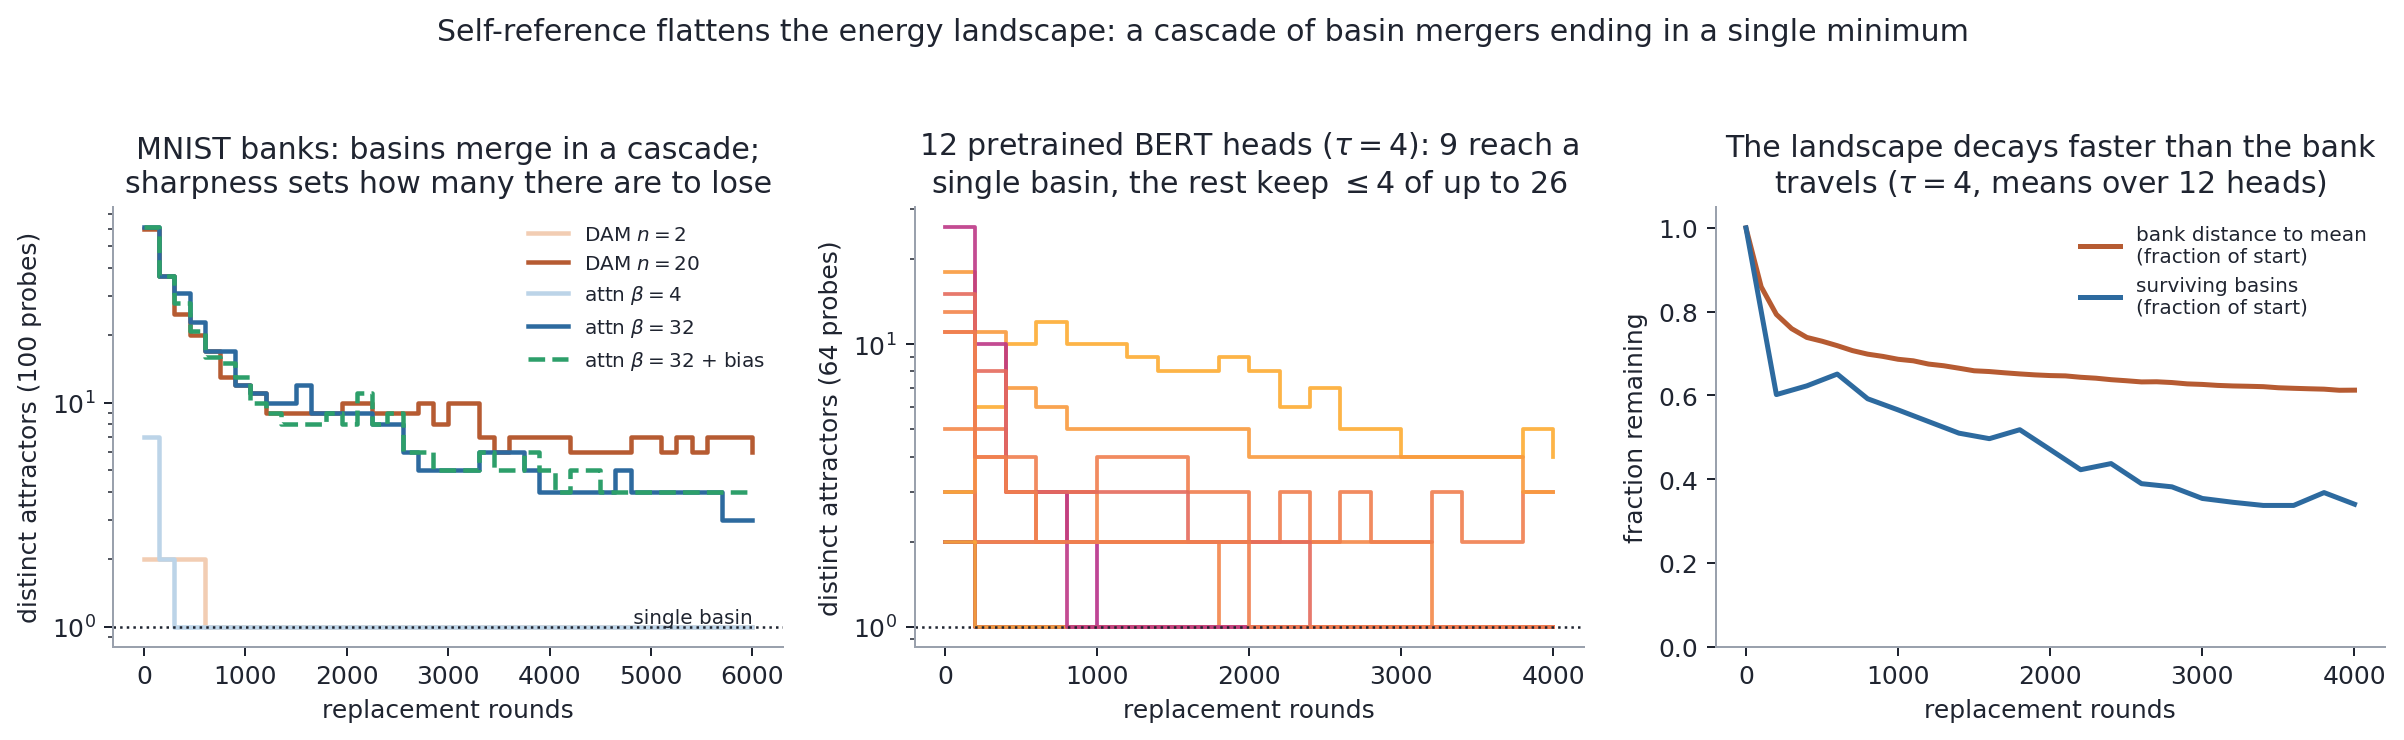
\includegraphics[width=\figwidth]{energy_flattening}
\caption{\textbf{Flattening, measured directly.} At fixed times the bank is
frozen and the retrieval map is iterated to convergence from a fixed set of
real probes; distinct limit points count the surviving basins. (a)~MNIST
banks: sharp rules start with $\sim$60 basins and lose them in a cascade;
blunt rules have almost none to lose. The energy-biased run (dashed)
tracks the unbiased cascade. (b)~The same census on pretrained BERT
retrieval maps ($\tau=4$): starting with up to 26 basins, nine of twelve
heads end with one, the rest with $\leq4$. (c)~Basins disappear faster
than the bank approaches the mean: the landscape loses its structure while
the patterns are still travelling.}
\label{fig:census}
\end{figure}

The statements above are consequences of a single geometric event, which I
measure directly: the number of attractors of the retrieval map, counted by
iterating the frozen map to convergence from fixed real probes and
de-duplicating the limit points. Sharp rules begin with many basins
($\sim$60 of 100 on MNIST at $\beta=32$ or $n=20$; up to 26 on sharpened
BERT heads) and lose them in a cascade of mergers; blunt rules begin
already nearly flat (Fig.~\ref{fig:census}a,b). The cascade outruns the
patterns themselves: at $\tau=4$ the surviving-basin fraction falls to a
third while the bank has covered barely 40\% of its distance to the mean
(Fig.~\ref{fig:census}c). The energy landscape dies first; the visible
drift of the patterns is the afterglow. This is the precise sense in which
``collapse'' is the right word: not a loss of data, but a loss of minima,
the heat death of a self-referential energy landscape.

\subsection{Three laws}

Across substrates (synthetic compositions, images, and pretrained
transformer hidden states) the same three regularities hold.

\textbf{Universal destination.} Unselected self-reference has one fixed
point. That it has a single one is guaranteed by
Proposition~\ref{prop:hull}; where it lies is not, and empirically it is a
single basin at (or drifting toward) the data mean, with uniform
attention. Prototype formation, the natural first guess, is falsified
pre-registeredly: averaging across retrievals beats averaging within
classes.

\textbf{Capacity is a clock, not a shield.} Interaction sharpness ($n$,
$\beta$, $\tau$) and initial regime position set every timescale in the
problem (exploration before fixation, capability half-life, basin
survival) and none of the destinations.

\textbf{Selection needs structure.} Basin-width selection converts the loop
from drift to discovery exactly when stored patterns encode a problem whose
recombinations can be externally better (spin glass), and merely slows the
clock when they do not (MNIST, BERT). By Proposition~\ref{prop:hull} the
two ingredients are distinct: a write that can leave the hull (here, the
binarizing projection) supplies novelty, and selection decides which
novelty is kept. Bias alone, applied to convex writes, can only choose
the order in which diversity is lost. The boundary between self-training
that collapses and self-training that discovers is a property of the task's
structure, not of the architecture's capacity.

\section{Discussion}

\textbf{An attractor account of model collapse.} The collapse of generative
models trained on their own outputs \citep{shumailov2024, alemohammad2024}
is usually described distributionally, as the loss of tails. Restricted to
the one module where the identity~(\ref{eq:identity}) is exact, I can
replace the description with a mechanism: self-reference couples an energy
landscape to its own minima, and the coupled system has a Lyapunov-like
one-way flow to the flat landscape. The known mitigations map cleanly:
accumulating rather than replacing data \citep{gerstgrasser2024} bounds the
fraction of self-written patterns; verification-based filtering is
selection with an external referee; and my basin-bias result sharpens the
requirement: similarity to real data is \emph{not} a sufficient referee,
because the mean is maximally similar to everything. Likewise the
convergence-to-the-prior of iterated learning \citep{griffiths2007} appears
here in its most stripped-down form: the ``prior'' of a retrieval map is
its uniform-attention fixed point.

\textbf{Relation to rank collapse.} Depth-wise rank collapse
\citep{dong2021, noci2022, geshkovski2025} and the self-referential
collapse reported here end at the same fixed point, uniform attention over
a single averaged pattern, but they differ in what moves. In rank collapse
the stored keys and values are recomputed at every layer from the tokens
of one input, and the collapse is a property of composing attention maps.
In self-reference a single map is applied repeatedly while its memory is
overwritten, and the collapse is a property of the memory, which persists
across inputs. Three observations follow. First, the remedies differ:
residual connections and normalization act on the forward pass
\citep{noci2022, wu2024} and have no counterpart in a store that is
rewritten in place; what slows my loop is sharpness, initial regime and
an external referee. Second, the clock is set by the same quantity in
both: sharper attention resists longer, whether measured in layers or in
rounds. Third, the basin census adds a statement the depth-wise analyses
do not make in energy terms: the attractors of the retrieval map vanish
before the patterns finish converging.

\textbf{For energy-based transformers.} Architectures that derive
transformer blocks from energies \citep{hoover2023} or spend inference
compute descending them \citep{gladstone2025} inherit an assumption of
landscape stationarity. My results are a first map of what happens when
that assumption is dropped at the memory level, as it is dropped in
practice wherever a retrieval store, cache, or training corpus is
populated by the system that reads it. The regime axis of
\citet{ramsauer2021} turns out to be not just a taxonomy but a flow line,
and position on it a survival time.

\textbf{When self-reference is worth having.} The spin-glass control
recovers, in modern form, the self-modeling effect of \citet{watson2011}
and the conditions of the self-optimization literature
\citep{froese2025}: self-reference adds value precisely when (i)~patterns
are compositional, so recombination can produce something new, and
(ii)~an external quality signal is allowed to shape basin geometry. Under
those two conditions the loop is a generate-and-test optimizer whose
generator is the memory itself; without them it is neutral drift with a
guaranteed flat endpoint.

\textbf{Limitations.} The contraction itself is a geometric certainty for
convex writes, so the contribution lies in its endpoint, its clock and its
basin dynamics rather than in the fact of collapse. These are small-scale,
mechanism-level experiments:
one pretrained model, banks of 100 patterns, retrieval-space dynamics
rather than full text generation, and BERT's asymmetric $W_Q W_K^{\top}$
means the head's iterated map is not literally gradient descent on a
symmetric energy (I therefore count attractors of the map, which is the
operationally relevant object). The pre-registered MNIST protocol also
taught me that my drift statistic cannot distinguish prototype formation
from mean formation in advance; only the controls made the verdict
unambiguous. Scaling the loop to generative language models, where the
bank is a KV cache or a corpus and the probe distribution itself shifts,
is the natural next experiment; the three laws above are its
pre-registered predictions.

\section{Methods}

\textbf{Retrieval rules.} Power rule (DAM): weights
$w_i\propto\max(\cos(q,x_i),0)^{\,n-1}$ \citep{krotov2016}; softmax rule
(attention): $w_i\propto\exp(\beta\cos(q,x_i))$ \citep{ramsauer2021}; both
applied to centred patterns, output $\mu + \sum_i w_i (x_i-\mu)$. On BERT
heads the logits are $\tau\,(qW_Q)(x_iW_K)^{\top}/\sqrt{64}$ with
pretrained weights and biases. Certification against the reference
implementation of \citet{ramsauer2021} used identity projections, static
patterns, and matched scaling.

\textbf{Spin-glass substrate.} Patterns are concatenations of $12$ module
configurations ($10$ alleles each) scoring against a frustrated coupling
matrix; the global optimum is known by exact enumeration. Self-training:
random valid query $\to$ retrieval $\to$ per-module binarization to the
nearest valid composition $\to$ overwrite a random slot with a $\delta$
mixture. Basin bias adds $-\gamma E_J(x_i)$ to the logits with $J$ frozen.
Grids: $\beta\in10^{0..3}$ (13 values) $\times$ $\delta$ (8 values)
$\times$ 6 seeds; selection arm $\beta\in\{10,\dots,1000\}\times
\gamma\in\{0,\dots,8\}\times10$ seeds.

\textbf{MNIST protocol.} Pre-registered before any run: the participation
ratio $\mathrm{PR}(\xi)=(\sum_i c_i^{+})^2/\sum_i (c_i^{+})^{2}$ of a
memory's positive correlation profile against 3{,}000 real images, validated
in advance on known cases (real images 2462 $<$ class means 2717 $<$
global mean 2899; random 1030); a difficulty check establishing that the
inpainting task needs memory rank 14--18 (ceiling 0.748, mean-image floor
0.130); then a $2\times4\times6\times6$ grid (rule $\times$ sharpness
$\times$ mode $\times$ seed), $K=100$, 6{,}000 replacement rounds, with
modes self, real-fed (C1), random-fed (C3), anchored (C4,
$\alpha\in\{0.99,0.90\}$) and an exploratory data-likeness bias
($\gamma=4$). Capability judged by masked-pixel reconstruction scored by a
1-NN classifier on held-out real images. Falsification criteria (monotone
PR decrease toward prototypes for H; non-monotone capability peak for
H$'$) were written in advance; both criteria fired negative, as reported.

\textbf{BERT experiment.} \texttt{bert-base-uncased}; token hidden states
from two public-domain books cached at layers 1, 5, 8, 11 (20{,}480
states per layer); per layer the most-averaging, median, and
most-selective heads by initial $k_{90}$ on a $K=100$ bank. Dynamics:
4{,}000 rounds $\times$ $\tau\in\{0.5,1,2,4\}$ $\times$ modes
\{self, real, random, bias\} $\times$ 4 seeds. Frozen probe set of 256
states; $k_{90}$, attention entropy, effective rank, distance to pool
mean, nearest-neighbour distance to real states, and distinct-slot count
recorded every 100 rounds at the head's native scale.

\textbf{Basin census.} At each stored time the bank is frozen and the
retrieval map iterated to convergence (tolerance $10^{-9}$ MNIST /
$10^{-5}$ BERT, $\leq300$ iterations) from fixed real probes (100 MNIST /
64 BERT); limit points are de-duplicated at cosine $0.999$.

\textbf{Statistics.} Per-seed units throughout; Mann--Whitney $U$ and
Cohen's $d$ for independent comparisons, Wilcoxon signed-rank for paired
ones, Spearman rank correlation for the half-life law. No statistic in the
abstract; all numbers in the text are means over seeds unless stated.

\section*{CRediT authorship contribution statement}
\textbf{Nam H. Le:} Conceptualization, Methodology, Software, Formal
analysis, Investigation, Visualization, Writing -- original draft, Writing
-- review \& editing.

\section*{Declaration of competing interest}
The author declares no known competing financial interests or
personal relationships that could have appeared to influence the work
reported in this paper.

\section*{Funding}
This research did not receive any specific grant from funding agencies in
the public, commercial, or not-for-profit sectors.

\section*{Declaration of generative AI and AI-assisted technologies in the writing process}
During the preparation of this work the author used generative AI tools in order to
draft and edit the text. After using these tools, the author reviewed and edited the
content as needed and takes full responsibility for the content of the published article.

\section*{Data availability}
All code, the stored results behind every figure, and the pre-registered
MNIST protocol are openly available at
\url{https://github.com/drnamlabs-gif/self-referential-attention}.

\begin{thebibliography}{99}

\bibitem[Alemohammad et al.(2024)]{alemohammad2024}
S.~Alemohammad, J.~Casco-Rodriguez, L.~Luzi, A.~I. Humayun, H.~Babaei,
D.~LeJeune, A.~Siahkoohi, and R.~Baraniuk.
\newblock Self-consuming generative models go {MAD}.
\newblock \emph{ICLR}, 2024.

\bibitem[Bertrand et al.(2024)]{bertrand2024}
Q.~Bertrand, A.~J. Bose, A.~Duplessis, M.~Jiralerspong, and G.~Gidel.
\newblock On the stability of iterative retraining of generative models on
their own data.
\newblock \emph{ICLR}, 2024.

\bibitem[DeGroot(1974)]{degroot1974}
M.~H. DeGroot.
\newblock Reaching a consensus.
\newblock \emph{Journal of the American Statistical Association},
69(345):118--121, 1974.

\bibitem[Demircigil et al.(2017)]{demircigil2017}
M.~Demircigil, J.~Heusel, M.~L{\"o}we, S.~Upgang, and F.~Vermet.
\newblock On a model of associative memory with huge storage capacity.
\newblock \emph{Journal of Statistical Physics}, 168:288--299, 2017.

\bibitem[Dong et al.(2021)]{dong2021}
Y.~Dong, J.-B. Cordonnier, and A.~Loukas.
\newblock Attention is not all you need: pure attention loses rank doubly
exponentially with depth.
\newblock In \emph{Proceedings of the 38th International Conference on
Machine Learning (ICML)}, PMLR 139, pages 2793--2803, 2021.

\bibitem[Froese et al.(2025)]{froese2025}
T.~Froese et~al.
\newblock Self-optimization in {Hopfield} neural networks: a review.
\newblock Review of the self-modeling/self-optimization literature, 2025.

\bibitem[Geshkovski et al.(2025)]{geshkovski2025}
B.~Geshkovski, C.~Letrouit, Y.~Polyanskiy, and P.~Rigollet.
\newblock A mathematical perspective on transformers.
\newblock \emph{Bulletin of the American Mathematical Society},
62:427--479, 2025.

\bibitem[Gerstgrasser et al.(2024)]{gerstgrasser2024}
M.~Gerstgrasser, R.~Schaeffer, A.~Dey, et~al.
\newblock Is model collapse inevitable? {Breaking} the curse of recursion by
accumulating real and synthetic data.
\newblock \emph{COLM}, 2024.

\bibitem[Gladstone et al.(2025)]{gladstone2025}
A.~Gladstone, G.~Nanduru, M.~S. Islam, et~al.
\newblock Energy-based transformers are scalable learners and thinkers.
\newblock \emph{arXiv:2507.02092}, 2025.

\bibitem[Griffiths and Kalish(2007)]{griffiths2007}
T.~L. Griffiths and M.~L. Kalish.
\newblock Language evolution by iterated learning with {Bayesian} agents.
\newblock \emph{Cognitive Science}, 31(3):441--480, 2007.

\bibitem[Hoover et al.(2023)]{hoover2023}
B.~Hoover, Y.~Liang, B.~Pham, R.~Panda, H.~Strobelt, D.~H. Chau, M.~J.
Zaki, and D.~Krotov.
\newblock Energy transformer.
\newblock \emph{NeurIPS}, 2023.

\bibitem[Hopfield(1982)]{hopfield1982}
J.~J. Hopfield.
\newblock Neural networks and physical systems with emergent collective
computational abilities.
\newblock \emph{PNAS}, 79(8):2554--2558, 1982.

\bibitem[Krotov and Hopfield(2016)]{krotov2016}
D.~Krotov and J.~J. Hopfield.
\newblock Dense associative memory for pattern recognition.
\newblock \emph{NeurIPS}, 2016.

\bibitem[Noci et al.(2022)]{noci2022}
L.~Noci, S.~Anagnostidis, L.~Biggio, A.~Orvieto, S.~P. Singh, and
A.~Lucchi.
\newblock Signal propagation in transformers: theoretical perspectives and
the role of rank collapse.
\newblock In \emph{Advances in Neural Information Processing Systems
(NeurIPS)}, volume~35, 2022.

\bibitem[Pham et al.(2025)]{pham2025}
B.~Pham, G.~Raya, M.~Negri, M.~J. Zaki, L.~Ambrogioni, and D.~Krotov.
\newblock Memorization to generalization: emergence of diffusion models
from associative memory.
\newblock \emph{arXiv:2505.21777}, 2025. Published in \emph{Nature
Communications}, 2026.

\bibitem[Ramsauer et al.(2021)]{ramsauer2021}
H.~Ramsauer, B.~Sch{\"a}fl, J.~Lehner, P.~Seidl, M.~Widrich, et~al.
\newblock Hopfield networks is all you need.
\newblock \emph{ICLR}, 2021.

\bibitem[Serricchio et al.(2025)]{serricchio2025}
L.~Serricchio, D.~Bocchi, C.~Chilin, R.~Marino, M.~Negri, C.~Cammarota, and
F.~Ricci-Tersenghi.
\newblock Daydreaming {H}opfield networks and their surprising
effectiveness on correlated data.
\newblock \emph{Neural Networks}, 186:107216, 2025.

\bibitem[Shumailov et al.(2024)]{shumailov2024}
I.~Shumailov, Z.~Shumaylov, Y.~Zhao, N.~Papernot, R.~Anderson, and
Y.~Gal.
\newblock {AI} models collapse when trained on recursively generated data.
\newblock \emph{Nature}, 631:755--759, 2024.

\bibitem[Takeda et al.(2026)]{takeda2026}
K.~Takeda, M.~Oizumi, and R.~Karakida.
\newblock Continual learning in modern {H}opfield networks with an
application to diffusion models.
\newblock \emph{arXiv:2605.27975}, 2026.

\bibitem[Vaswani et al.(2017)]{vaswani2017}
A.~Vaswani, N.~Shazeer, N.~Parmar, J.~Uszkoreit, L.~Jones, A.~N. Gomez,
{\L}.~Kaiser, and I.~Polosukhin.
\newblock Attention is all you need.
\newblock \emph{NeurIPS}, 2017.

\bibitem[Wu et al.(2024)]{wu2024}
X.~Wu, A.~Ajorlou, Y.~Wang, S.~Jegelka, and A.~Jadbabaie.
\newblock On the role of attention masks and {L}ayer{N}orm in
transformers.
\newblock In \emph{Advances in Neural Information Processing Systems
(NeurIPS)}, 2024.

\bibitem[Watson et al.(2011)]{watson2011}
R.~A. Watson, C.~L. Buckley, and R.~Mills.
\newblock Optimization in ``self-modeling'' complex adaptive systems.
\newblock \emph{Complexity}, 16(5):17--26, 2011.

\end{thebibliography}

\end{document}
